\documentclass[a4paper,12pt, oneside]{book}

%\usepackage{fullpage}
\usepackage[T1]{fontenc}
\usepackage[italian]{babel}
\usepackage[utf8]{inputenc}
\usepackage{amssymb}
\usepackage{amsthm}
\usepackage{graphics}
\usepackage{amsfonts}
\usepackage{listings}
\usepackage{amsmath}
\usepackage{amstext}
\usepackage{engrec}
\usepackage{rotating}
\usepackage[safe,extra]{tipa}
\usepackage{showkeys}
\usepackage{multirow}
\usepackage{hyperref}
\usepackage{microtype}
\usepackage{enumerate}
\usepackage{braket}
\usepackage{marginnote}
\usepackage{pgfplots}
\usepackage{cancel}
\usepackage{polynom}
\usepackage{booktabs}
\usepackage{enumitem}
\usepackage{framed}
\usepackage{pdfpages}
\usepackage{pgfplots}
\usepackage[usenames,dvipsnames]{pstricks}
\usepackage{epsfig}
\usepackage{pst-grad} % For gradients
\usepackage{pst-plot} % For axes
\usepackage[space]{grffile} % For spaces in paths
\usepackage{etoolbox} % For spaces in paths
\makeatletter % For spaces in paths
\patchcmd\Gread@eps{\@inputcheck#1 }{\@inputcheck"#1"\relax}{}{}
\makeatother
\usepackage[cache=false]{minted}
\usepackage{fancyhdr}
\newcommand{\numberset}{\mathbb}
\newcommand{\N}{\numberset{N}}
\newcommand{\Z}{\numberset{Z}}
\newcommand{\Q}{\numberset{Q}}
\newcommand{\R}{\numberset{R}}

\pagestyle{fancy}
\fancyhead[LE,RO]{\slshape \rightmark}
\fancyhead[LO,RE]{\slshape \leftmark}
\fancyfoot[C]{\thepage}



\title{Probabilità e Statistica per l'Informatica}
\author{UniShare\\\\Davide Cozzi\\\href{https://t.me/dlcgold}{@dlcgold}\\\\Gabriele De Rosa\\\href{https://t.me/derogab}{@derogab} \\\\Federica Di Lauro\\\href{https://t.me/f_dila}{@f\textunderscore dila}}
\date{}

\pgfplotsset{compat=1.13}
\begin{document}
\maketitle
\tableofcontents

\definecolor{shadecolor}{gray}{0.80}

\newtheorem{teorema}{Teorema}
\newtheorem{definizione}{Definizione}
\newtheorem{esempio}{Esempio}
\newtheorem{corollario}{Corollario}
\newtheorem{lemma}{Lemma}
\newtheorem{osservazione}{Osservazione}
\newtheorem{nota}{Nota}
\newtheorem{esercizio}{Esercizio}
\newcommand{\mean}[1]{\overline #1}
\renewcommand{\chaptermark}[1]{%
\markboth{\chaptername
\ \thechapter.\ #1}{}}
\renewcommand{\sectionmark}[1]{\markright{\thesection.\ #1}}
\chapter{Introduzione}
\textbf{Questi appunti sono presi a lezione. Per quanto sia stata fatta una revisione è altamente probabile (praticamente certo) che possano contenere errori, sia di stampa che di vero e proprio contenuto. Per eventuali proposte di correzione effettuare una pull request. Link: } \url{https://github.com/dlcgold/Appunti}.\\
\textbf{Grazie mille e buono studio!}
\chapter{Breve Introduzione}
La statistica è una discliplina, basata sulla matematica, con il fine lo studio quantitativo e qualitativo
di un particolare fenomeno collettivo in condizioni di incertezza o non determinismo ed è usata in molti 
ambiti come ad esempio l'intelligenza artificiale, data science, robotica, domotica e tutte le analisi 
per poter ottenere ricavare delle informazioni sui dati.

Ormai i dati sono pervasivi e un loro studio è diventato necessario ed inoltre si parla spesso di target marketing,
con una selezione dei possibili clienti infatti è usata in maniera massiccia nel mondo dello shopping online.\newline
Si ha l'\textit{A-B testing}, per decidere tra due scelte la migliore e per la decisione si analizzano i dati
presi da campioni di popolazione, utilizzando il \textit{tasso di conversione}, ossia la percentuale di visitatori unici
che hanno effettuato la azione su cui si sta effettuando il test.

In codesto corso vengono effettuati i seguenti argomenti:
\begin{enumerate}
    \item statistica descrittiva
    \item calcolo delle probabilità
    \item distribuzioni notevoli
    \item teoremi di convergenza
    \item stima dei parametri
    \item test di ipotesi parametrici
    \item test di ipotesi non parametrici
    \item regressione lineare
\end{enumerate}

\chapter{Statistica Descrittiva}
La statistica descrittiva è una raccolta di metodi e strumenti matematici usati per organizzare una o più serie di dati
al fine di trovarne delle simmetrie, periodicità o delle eventuali leggi, ossia si effettua una descrizione 
delle informazioni implicite ai dati.

Solitamente i dati disponibili non rappresentano tutta la popolazione ma un numero limitato 
di osservazioni effettuato su un \emph{campione}, sottoinsieme selezionato della popolazione su cui si effettua
l'analisi statistica, la cui efficacia rispetto alla popolazione dipende da quale sottoinsieme è stato scelto
infatti non esiste un solo campione ma vi sono diversi modi per sceglierli, più o meno efficaci, per l'analisi statistica.

Quando si effettua un analisi statistica si vuole affermare qualcosa riguardo i \textbf{caratteri} della popolazione,
ossia gli elementi su cui effettuo l'analisi statistica, che possono essere:
\begin{itemize}
    \item \textbf{caratteri qualitativi}, indicanti qualità (colori, stili, materiali etc...) e anche dati non numerici
             in cui solitamente non è definita una \textit{relazione d'ordine}
    \item \textbf{caratteri quantitativi}, maggiormente studiati dal corso, dati numerici in cui vengono definite \emph{relazioni d'ordine}:
        \begin{itemize}
            \item \textbf{discreti}, come i lanci di un dado, rappresentanti valori in $\Z$
            \item \textbf{continui}, che assumono valori reali, come la temperatura, in $\R$
        \end{itemize}
\end{itemize}
Supponiamo di considerare $n$ elementi della popolazione e di rilevare, per ognuno di essi,
il dato relativo al carattere quantitativo da esaminare, ossia definiamo l'insieme di dati
$E=\{x_1, x_2, \dots, x_n\}$ con la numerosità, il numero di elementi considerati, pari a $n$.

In caso il carattere è quantitativo discreto è comodo raggruppare i dati considerando 
l'insieme di tutti i valori assumibili, detta \textbf{modalità del carattere} ed associare ad ognuno 
di esso il numero di volte che esso compare in $E$.\newline
Si ha quindi $N$ il numero di totalità del carattere e si definisce l'insieme di modalita
$S=\{s_1,...,s_N\}$ su cui si definiscono i seguenti valori statistici:
\begin{description}
    \item [frequenza assoluta $f_j$] numero di volte che si presenta un elemento di un campione
    \item [frequenza cumulata assoluta $F_j$] somma delle frequenze assolute di tutte le modalità:
            \[ F_j = \sum_{k:s_k \leq s_j} f_k \]
    \item [frequenza relativa $p_j$] rapporto tra la frequenza assoluta e il numero di elementi 
            \[ p_j = \frac{f_j}{n} \]
    \item [frequenza cumulativa relativa $P_j$] somma delle frequenze relativa di tutte le modalità:
            \[ P_j = \sum{k:s_k \leq s_j} p_k \]
\end{description}
Si definisce \textbf{distribuzione di frequenza} una funzione $F:S \to \N$ che associa ad ogni modalità la corrispondente frequenza
per cui esiste la distribuzione di frequenza assoluta, relativa, frequenza cumulativa assoluta e relativa.

%inserire esempio pagina 9
Quando il carattere da studiare è continuo (o discreto con un gran numero di valori) è conveniente 
ricondursi a raggruppamenti come quelli appena trattati, per cui si suddivide $S$, l'insieme delle modalità,
in alcune classi (sottoinsiemi di $S$) che formano una partizione e la scelta delle classi con cui 
si suddivide l'insieme $S$ è del tutto arbitraria anche se è necessario che esse formino una partizione di $S$.\newline
Le partizioni devono essere significative e sufficientemente numerose ed inoltre ad ogni classe si associano le grandezze:
\begin{itemize}
\item confine superiore e inferiore (valori estremi della classe)
\item ampiezza (differenza tra confine superiore ed inferiore)
\item valore centrale (media tra i due confini)
\end{itemize}
Nel caso in cui il carattere esaminato sia continuo occorre specificare come le classi sono chiuse, a destra o a sinistra,
ossia specificare se gli elementi dell'indagine il cui dato coincide con il confine della classe sono da raggruppare
all'interno della classe stessa oppure no.
%esempio a pagina 13
\section{Indici di tendenza Generale}
Fino ad ora abbiamo visto come rappresentare i dati, sia discreti che continui, ora iniziamo ad analizzare gli indici
che ci forniscono un valore che rappresenta un certo aspetto della serie di dati, 
incominciando dagli \textbf{indici di tendenza generale}:
\begin{description}
    \item [media] è la media aritmetica tra tutti i valori dei dati osservati 
            \[ \overline{x} = \frac{1}{n} \sum x_i = \frac{x_1 + \cdots + x_n}{n} \]
            Considerando le distribuzioni di frequenza definite, posssiamo fornire definizioni equivalenti di media:
                \[ \overline{x} = \frac{1}{n} \sum s_j f_j = \sum s_j p_j \]
                La dimostrazione dell'uguaglianza di queste definizioni alternative è banale e si riconduce 
                alla definizione di frequenza relativa ed assoluta.

    \item [mediana] è l'elemento in mezzo ai valori dei dati, ordinati in maniera crescente
            in cui se il numero degli elementi $n$ è dispari è l'elemento $\frac{n + 1}{2}$
            altrimenti è la somma degli elementi di posto $\frac{n}{2}$ e $\frac{n}{2} + 1$.

    \item [moda $\widetilde{x}$] valore o classe corrispondente alla massima frequenza assoluta e viene usata 
            solitamente in caso sia impossibile definire la media e la mediana.\newline
            La moda non è unica infatti parliamo di:
            \begin{itemize}
                 \item \textbf{distribuzione uni-modale} nel caso in cui vi sia un unica moda
                 \item \textbf{distribuzione multi-modale} nel caso in cui vi siano più mode
            \end{itemize}
\end{description}
%aggiungo esempio
Gli indici di tendenza centrale non sono utili per fornire informazioni circa l'omogeneità dei dati in quanto forniscono 
informazioni sui valori centrali e medi del campione statistico per cui per risolvere sto problema introduciamo i seguenti indici:
\begin{description}
        \item [varianza] è la media dello scarto quadratico di ogni elemento dalla sua media 
                \[ s^2 = \frac{1}{n} \sum _{i = 1} ^ n (x_i - \overline{x})^2 \]
                La varianza ovviamente è tanto più grande quanto i singoli elementi si discostano dalla media, 
                ossia significa che i dati in tal caso sono molto disomogenei.
                Come abbiamo già visto per la media sono presenti le seguenti definizioni alternative di varianza:
                \[ s^2 = \frac{1}{n} \sum _{j = 1} ^ N f_j (s_j - \overline{x}) ^ 2 \]
                \[ s^2 = \sum _{j = 1} ^ N p_j (s_j - \overline{x}) ^ 2 \]
                \[ s^2 = \sum _{j = 1} ^ n x_j - \overline{x} ^ 2 \]
                Le prime due definizioni alternative derivano dalla definizione di frequenza assoluta e frequenza 
                mentre l'ultima proviene da passaggi algebrici, dimostrati di seguito formalmente:
                \begin{proof}
                        \[ \begin{split}
                            s^2 & = \frac{1}{n} \sum _{i = 1} ^ n (x_i - \mean{x}) ^ 2 \\
                                & = \frac{1}{n} \sum (x_i ^ 2 - 2x_i\mean{x} + \mean{x} ^ 2) \\
                                & = \frac{1}{n} (\sum x_i^2 - 2\mean{x} \sum x_i + \sum \mean{x} ^ 2) \\
                                & = \frac{1}{n} (\sum x_i^2 - 2n\mean{x}^2 + n\mean{x}^2) \\
                                & = \frac{1}{n} \sum x_i^2 - \mean{x} ^ 2 \\
                            \end{split} \]
                Si dimostra $\sum x_i = n \mean{x}$ in quanto $\mean{x} = \frac{1}{n} \sum x_i$ e il resto 
                sono soltanto passaggi algebrici elementari
                \end{proof}

    \item [scarto quadratico medio] misura quanto sono distanti gli elementi di un campione ed è calcolata come:
            \[ s = \sqrt{s^2} = \sqrt{\frac{1}{n} \sum _{i = 1} ^ n (x_i - \overline{x}) ^ 2} \]
\end{description}
Nel calcolo della varianza si utilizza il quadrato per la differenza tra l'elemento e la sua media in quanto 
per come è definita la media si ha $\sum (x_i - \overline{x}) = 0$ e per evitare ciò si eleva la differenza 
tra un elemento e la sua media al quadrato.

La varianza è definito come il momento secondo rispetto alla media, espresso tramite la formula:
\[ M_{k,y}=\frac{1}{n}\sum (x_i-y)^2 \]

\section{Il caso bidimensionale}
Fino ad ora noi abbiamo considerato il caso unidimensionale in cui consideriamo solo un carattere del campione ma 
molte analisi richiedono di analizzare due o più caratteri del campione contemporaneamente, per riconoscere 
leggi ed analogie tra i diversi caratteri.\newline
Considereremo solo due caratteri contemporanei, sia perché un analisi con più caratteri si comporta uguale e sia 
per non aggravare troppo la rappresentazione dei dati negli esempi e assumiamo che entrambi i caratteri sono di
tipo quantitativo e discreto, in quanto se fossero quantitativi continui subirebbero prima un raggruppamento a classi.

L'insieme dei dati viene rappresentato come l'insieme delle coppie
\[ E = \{(x_1, y_1), (x_2, y_2) \dots, (x_n, y_n)\} \]
mentre l'insieme delle coppie di valori assumibili si rappresentati con l'insieme
\[ S = \{(s_j, u_k), \, j = 1 \dots N \quad k = 1 \dots M\} \]
Come abbiamo fatto anche per il caso unidimensionale definiamo le seguenti quantità:
\begin{description}
    \item [frequenza assoluta $(s_j, u_k)$] è la quantita $f_{jk}$ corrispondente al numero di elementi con valore $(s_j, u_k)$
    \item [frequenza relativa] \[ p_{jk} = \frac{f_{jk}}{n} \] rapporto tra la frequenza e il numero di elementi
    \item [frequenza cumulata assoluta]  \[ F_{jk} = \sum _{r:s_r \leq s_j; l:u_l \leq u_k} f_{rl} \]
    \item [frequenza cumulata relativa] \[ P_{jk} = \sum _{r:s_r \leq s_j; u_l \leq u_k} p_{rl} \] frequenza 
\end{description}
Si definisce \emph{distribuzione di frequenza doppia} una qualsiasi funzione $f, F, p, P$ 
che associa ad ogni coppia $(s_j, u_k)$ la corrispondente frequenza ma esistono anche altri tipi di distribuzioni,
infatti noi vediamo le \textbf{distribuzioni marginali}: distribuzioni dei singoli caratteri presi indipendemente degli altri.

Le distribuzioni marginali hanno la definizione delle seguenti funzioni:
\begin{description}
    \item [frequenza assoluta marginale] quantità di elementi $f_xj$ data dagli elementi di $E$, il cui primo carattere ha valore $s_j$
    \item [frequenza relativa marginale] rapporto tra la frequenza assoluta marginale e il numero di osservazioni $n$.
    \item [frequenza cumulata assoluta marginale] $F_{xj}$ somma delle frequenze assolute marginali di tutti gli $s_k$ con $s_k \leq s_j$
    \item [frequenza cumulata relativa marginale] $P_{xj}$ somma delle frequenze relative marginali di tutti gli $s_k$ con $s_k \leq s_j$
\end{description}
Oltre agli indici definiti fino ad ora, esiste un indice che fornisce un grado di interdipendenza tra i due caratteri,
indice importante in quanto molti problemi concreti necessitano di analizzare gradi di correlazione tra due o più serie di dati,
iniziando prima di tutto da un esempio.

Considero due serie $\{x_i\},\{y_i\},\,\,i=1,...,n$ ponendo a confronto le variazione delle coppie di dati
rispetto ai corrispondenti valori medi, considerando le coppie di scarti:
\[ x_i - \overline{x} \]
\[ y_i - \overline{y} \]
si ha una relazione di dipendenza tra i due caratteri se i due scarti corrispondono sistematicamente o quasi valori positivi o negativi.

Si definisce quindi la \textbf{covarianza} $c_{xy}$, dei dati o campionaria, delle due serie di dati :
\[ c_{xy} = \frac{1}{n} \sum (x_i - \overline{x}) (y_i - \overline{y}) \]
La covarianza assume un valore positivo (negativo) che diviene grande in valore assoluto nel caso in cui 
i termini prodotto abbiano segni concordi e in questo caso si parla di serie statistiche fortemente correlate
o per meglio dire di dati delle serie fortemente correlati.\newline
Nel caso opposto vale a dire nel caso in cui i dati delle serie siano incorrelati avremo che i prodotti
avranno segni diversi (saranno discordi in segno) e la covarianza, per come definita,
risulterà piccola in valore assoluto, prossima al valore 0.

Si ha anche la seguente formula per la covarianza:
\[ c_{xy} = \frac{1}{n} \sum x_iy_i - \overline{x}\overline{y} \]
\begin{proof}
        \[ \begin{split}
                c_{xy} & = \frac{1}{n} \sum _{i = 1} ^ n (x_i - \mean{x}) (y_i - \mean{y}) \\
                       & = \frac{1}{n} \sum _{i = 1} ^ n (x_iy_i - x_i\mean{y} - y_i \mean{x} + \mean{x}\mean{y}) \\
                       & = \frac{1}{n} (\sum x_iy_i - \mean{y} \sum x_i - \mean{x} \sum y_i + \sum \mean{x}\mean{y}) \\
                       & = \frac{1}{n} (\sum x_iy_i - n\mean{y}\mean{x} - n\mean{y}\mean{x} + n\mean{y}\mean{x}) \\
                       & = \frac{1}{n} (\sum x_iy_i - n\mean{x}\mean{y}) \\
                       & = \frac{1}{n} \sum x_iy_i - \mean{x}\mean{y} \\
            \end{split} \]
\end{proof}
Nel caso in cui i dati si riferiscano a caratteri quantitativi discreti, di cui è nota la
distribuzione di frequenza doppia, è possibile utilizzare le seguenti formule per il calcolo della covarianza:
\[ c{xy}=\sum_1^N\sum_1^M(s_j-\overline{x})(u_k-\overline{y})p_{jk} \]
\[c{xy}=\sum_1^N\sum_1^Ms_ju_kp_{jk}-\overline{x}\overline{y} \]

Date due serie di dati si ha che sono:
\begin{itemize}
    \item \textbf{statisticamente incorrelate} se la loro covarianza è nulla
    \item \textbf{statisticamente indipendenti} se vale:
        \[ \forall j=1, \dots, N\,\,k=1, \dots, M\,\,\, p_{jk} = p_jp_k \]
             con:
            \[ p_{jk}=\frac{f_{jk}}{n} \]
            \[ p_{j}=\frac{f_{j}}{n} \]
            \[ p_{k}=\frac{f_{k}}{n} \]        
\end{itemize}
inoltre due serie di dati statisticamente indipendenti sono incorrelate mentre non è necessariamente vero il contrario, infatti:
\[ \sum \sum (x_i - \overline{x})(y_i - \overline{y}) = \sum (x_i - \overline{x}) \sum(y_i - \overline{y}) = 0 \]
Nel caso bidimensionale, con variabili x e y, la covarianza si può rappresentare attraverso una matrice $2 \times 2$:
\[ C = \left | \begin{matrix}
                c_{xx} & c_{xy}\\
                c_{xy} & c_	{yy}
                \end{matrix}\right| = \left|\begin{matrix}
                                            var(x) & cov(x,y)\\
                                            cov(x,y) & var(y)
                                            \end{matrix}\right| \]
Per una misura indipendente dalla variabilità delle grandezze si usa la matrice di correlazione:
\[ Corr=\left|\begin{matrix}
              \frac{c_{xx}}{\sigma_x^2} & \frac{c_{xy}}{\sigma_x^2\sigma_y^2} \\
              \frac{c_{xy}}{\sigma_x^2\sigma_y^2}   & \frac{c_{yy}}{\sigma_y^2} 
              \end{matrix}\right|=\left|\begin{matrix}
                                            1 & corr(x,y)\\
                                            corr(x,y) & 1
                                        \end{matrix}\right| \]
che ovviamente può crescere in $m$ dimensioni.

\section{Regressione Lineare}
La regressione lineare 

Prendo un campione di coppie di dati:
\[ E = \{(x_1,y_1), \dots, (x_n,y_n)\} \]
In molti casi ci si pone la questione se tra tali caratteri $x$ ed $y$ esista un legame di tipo funzionale
o una relazione di tipo funzionale che ne descriva in modo soddisfacente corretto il legame realmente esistente.\newline
Si parla di un'\textbf{analisi di regressione}, in cui si pensa ad uno dei due caratteri come variabile indipendente e
si cerca una funzione che stabilisce la relazione tra i due caratteri.\newline
Se fisso $x$, come \textbf{variabile indipendente}, cerco $y = f(x)$ in modo che essa descriva al meglio
il legame tra la variabile indipendente $x$ e il carattere $y$ che a questo punto viene interpretato come \textbf{variabile dipendente}.

Si determina quindi la funzione $f$ che minimizza le distanze tra i valori osservati del carattere $y$
e quelli che si otterrebbero per il carattere $y$ se la relazione che lega il carattere $y$ ad $x$ 
fosse proprio quella descritta da $f$, quindi cerco la funzione $f$ che minimizza la quantità:
\[ g(f) = \sum[f(x_i)-y_i]^2 \]
dove il quadrato si utilizza affinché le distanze vengano tutte considerate con segno positivo.\newline
Se $f$ è vincolata ad essere una funzione lineare allora si parla di \textbf{regressione lineare}, con la retta rappresentata da:
\[ y=mx+q \]
con $q$ intercetta e $m$ coefficiente angolare, tale per cui risulti minima la quantità:
\[ g(m,q) = \sum[mx_i+q-y_i]^2 \]
con $mx_i+q=f(x_i)$ che sono l'approssimazione alle $y_i$ mediante $f$. Si ha che:
\[ m = \frac{c_{xy}}{s^2_x} \]
\[ q = \overline{y} - \frac{c_{xy}}{s_x^2}\overline{x} \]
Questo metodo consente di determinare la retta che meglio descrive la relazione tra i due caratteri 
senza peraltro fornire alcuna indicazione circa il grado di approssimazione che è in grado di offrire.\newline
Per tale motivo è stata introdotta una nuova grandezza detta \textbf{coefficiente di correlazione lineare:}
\[ r_{xy}=\frac{c_{xy}}{s_xs_y} \]
L'importanza di tale coefficiente deriva dal fatto che esso assume valori sempre appartenenti all'intervallo $[-1, 1]$ 
ed inoltre è nullo se le serie sono statisticamente incorrelate; il valore assoluto risulta tendente a 1
se le coppie sono tutte sulla retta $y=mx+q$ quindi rappresenta il grado di allineamento delle coppie di dati

\section{Regressione non Lineare}
Abbiamo accennato in precedenza al fatto che non si è sempre vincolati alla scelta di una retta tra le funzioni
che possono descrivere la relazione tra le due serie di dati ma quanto esposto in precedenza può essere applicato 
anche nel caso in cui si considerino relazioni funzionali di diversa natura, la cui scelta può essere suggerita
da una qualche impressione derivante da ispezioni visive dei dati o da altre forme di conoscenza circa il fenomeno analizzato,
avendo quindi il modello non lineare di regressione.

Molte relazioni funzionali non lineari possono essere ricondotte a tali (lineari) con opportune trasformazioni delle variabili,
infatti prendendo per esempio la relazione:
\[ y = a\cdot e^{bx} \]
che si può riscrivere come:
\[ \widetilde{y} = \beta\cdot \widetilde{x}+\alpha \]
con: 
\[ \widetilde{y}=\log(y) \]
\[ \widetilde{x}=x \]
\[ \alpha=\log(a) \]
\[ \beta = b \]
si ottiene quindi una sorta di curva e non più una retta.

La determinazione dei coefficienti a e b che meglio permettono di approssimare una serie di punti $\{x_i,y_i\}$ 
può essere effettuata riconducendosi ad una regressione lineare ovvero determinando i coefficienti $\alpha,\beta$ 
che meglio approssimano, linearmente, la serie dei punti $\{\widetilde{x}_i,\widetilde{y}_i\}$, con:
\[ \widetilde{y}_i = \log(y_i) \]
\[ \widetilde{x}_i = x_i \]
Una volta determina ti tali coefficienti il calcolo di $a$ e $b$ risulta immediato. 

Ecco alcune funzioni riconducibili a lineari:
\[ y = a \log(x) + b \]
\[ y=ax^b \]
\[ y=\frac{1}{a+b\cdot e^{-x}} \]

\chapter{Calcolo delle probabilità}
Disciplina di carattere matematico che permette di affrontare l'analisi delle situazioni che hanno un esito imprevedibile
a priori e pertanto con conseguenze incerte ed è lo strumento di base della statistica, che invece trae conclusioni
su una popolazione, utilizzando i dati osservati su una collezione di individui appartenenti alla popolazione:
estraendo un conveniente campione e analizzandolo, si spera di poter trarre conclusioni circa l'intero infatti 
da un campione traggo un'inferenza riguardo la popolazione.

Si hanno 4 impostazioni per la probabilità:
\begin{enumerate}
    \item classica
    \item frequentista
    \item soggettivista
    \item assiomatica
\end{enumerate}
Iniziamo a considerare l'impostazione assiomatica, supponendo di voler studiare una situazione con un insieme $\Omega$
di possibili esiti ben distinti tra loro, detto \emph{spazio campione}, in cui tutti i suoi sottoinsiemi
$A$ sono eventi(elementari in caso contengono solo un elemento altrimenti sono eventi composti)
e ad ogni evento si ha una quantità numerica $P(A)$ detta probabilità.

Un passo fondamentale nel superare le polemiche sull'interpretazione del concetto di probabilità
fu compiuto da Kolmogorov (1933) che abbandonò il tentativo di fondare la teoria della probabilità su una 
interpretazione sperimentale del concetto e costruire una teoria secondo una \textbf{impostazione assiomatica},
trascendendo il significato effettivo di probabilità, rinviandone l'interpretazione al momento delle applicazioni.

Due eventi sono \textbf{incompatibili} se non hanno elementi in comune, formando un intersezione vuota
e l'insieme delle parti di $\Omega$, $\wp(\Omega)$, definisce ovviamente l'insieme di tutti i sottoinsiemi;
la probabilità deve essere definita per tutti gli elementi di $\wp(\Omega)$ con particolari proprietà (algebre di Boole o $\sigma$-algebre).

Si dice \textbf{misura di probabilità} ogni applicazione $P: \wp(\Omega) \to \R_0 ^ +$
che associa un valore reale ad ogni sottoinsieme di $\Omega$ e per cui valgono le seguenti proprietà:
\begin{itemize}
        \item $\forall A\subseteq \Omega$ esiste ed è un unico numero $P(A) \geq 0$
              Interpretando $P(A)$ come frequenza relativa dell'evento A, essa è compresa tra 0 e 1.

        \item $P(\Omega) = 1$ La probabilità che qualsiasi evento si realizzi sia in $\Omega$ è 1
        \item data la famiglia $\{A_i\in I\subseteq N\}$ di eventi incompatibili vale:
                \[ P\left(\bigcup_{i\in I}A_i\right) = \sum_{i\in I} P(A_i) \]
              ossia la probabilità che si verifichi uno qualsiasi degli eventi appartenenti ad un insieme
                di eventi incompatibili è data dalla somma delle probabilità del verificarsi di ogni evento 
                appartenente all'insieme di eventi incompatibili considerato.
\end{itemize}
Ogni misura di probabilità è una funzione che assegna valori numerici a sottoinsiemi di $\Omega$
e non ai suoi elementi (eventi elementari), come contrariamente si è portati a credere intuitivamente infatti
la funzione di misura di probabilità associa un valore agli eventi elementi 
come una conseguenza dell'assegnazione di valori ad eventi composti.\newline
La definizione di probabilità non fornisce indicazioni su quali valori numerici devono essere assegnati dato che dipende,
come sempre dal particolare problema da analizzare.

Dalla definizione assiomatica derivano facilmente le seguenti proprietà aggiuntive:
\begin{definizione}
Sia P una misura di probabilità definita sull'insieme delle parti $\wp(\Omega)$ di uno
spazio campione $\Omega$ ( $\overline{A}$ evento complementare di $A$ cioè somma di probabilità
pari a 1) allora:
    \begin{itemize}
        \item $\forall A,B\subseteq \Omega \mbox{ anche incompatibili }$\\ $\to P(A\cup B)=P(A)+P(B)-P(A\cap B)$
                %aggiungi mega dimostrazione
                \begin{proof}
                 Si dimostra che:
                \[ P(A \cup B) = P(A \cap \overline{B}) + P(A \cap B) + P(\overline{A} \cap B)\]
                 Si ricava e si sa che sono soddisfatte le seguenti equazioni
                 \[P(A) = P(A \cap \overline{B}) + P(A \cap B) \]
                 \[P(B) = P(A \cap B) + P(\overline{A} \cap B) \]
                        quindi si ricava dall'equazione iniziale, sostituendo $P(A)$ e $P(B)$ la seguente equazione:
                    \[P(A \cup B) = P(A) + P(B) - P(A \cap B)\]
                \end{proof}
        \item $\forall A\subseteq \Omega \to P(\overline{A})=1-P(A)$
              \begin{proof}
                    \[  \forall A\subseteq \Omega \to P(\overline{A})=1-P(A)\]
                        \[\downarrow\]
                    \[ 1 = P(A \cup \overline{A} = P(A) + P(\overline{A}) - P(A \cap \overline{A}) = P(A) + P(\overline{A}) - 0\]
              \end{proof}
        \item $\forall A\subseteq \Omega \to P(A)\leq 1$
        \item $\forall A,B\subseteq \Omega, A\subseteq B \to P(A)\leq P(B)$
    \end{itemize}
\end{definizione}
si ha che il terzo assioma della probabilità generalizza la definizione della $P(A \cup B)$,
nel caso di tutti gli eventi incompatibili mentre la terza e la quarta proprietà si dimostrano facilmente,
considerando gli elementi basilari di teoria degli insiemi e dei 3 assiomi della probabilità.

Si ha uno \textbf{spazi campione con elementi equiprobabili} se dato $\Omega = \{1, 2, \dots, N\}$ tale che:
\[P(\{1\}) = \dots = P(\{N\}) = p \]
Da questa formula si ricava facilmente le seguenti due equazioni, fondamentali per il calcolo della probabilità:
\[P(\{1\}) + \dots + P(\{N\}) = Np = p(\omega) = 1\]
\[P(\{i\}) = p = \frac{1}{n}\]
Da quest'ultima equazione, considerando anche il terzo assioma della probabilità si ricava che la probabilità
di evento $E$ è data dalla equazione $P(E) = \frac{\mbox{num. eventi elementari dell'evento} \, E}{N}$,
ossia se tutti gli eventi elementari sono equiprobabili, la probabilità di un evento E è
la proporzione degli eventi elementari dello spazio campione $\Omega$ che appartengono ad E.

Si ha la seguente \textbf{regola di calcolo}:\\
Si facciano due esperimenti. Se l'esperimento 1 può avere n
possibili esiti equiprobabili, e l'esperimento 2 può avere m possibili esiti equiprobabili, allora i
due esperimenti insieme hanno $n\times m$ possibili esiti.
%aggiungere dimostrazione
Se si espande a $r$ esperimenti si avranno $n_1\times n_2\times ...\times n_r$ possibili esiti.
\section{Coefficiente Binomiale}
Una \textbf{permutazione} è un ordinamento senza ripetizione di simboli.\\
Si voglia determinare il numero di differenti gruppi di r oggetti che è possibile costruire
(formare) usando n oggetti diversi (non importa l’ordine degli oggetti). Si ottiene che:
\[\frac{n(n-1)...(n-r+1)}{r!}=\frac{n!}{(n-r)!\,r!}= {n\choose r}\]
detto \textbf{coefficiente binomiale}, ovvero il numero delle combinazioni di $n$ oggetti presi a gruppi di $r$.\\
Si ha inoltre che:
\[P(E)=\frac{\mbox{num eventi elementari} \, E}{N}\]
se ho più casi faccio:
\[P=\frac{modo_1\cdot modo_2}{tutti\,\, i\,\, possibili\,\, gruppi}\]

\section{Probabilità condizionata}
In molti casi, quando si desideri studiare un fenomeno con comportamenti aleatori, oppure si vuole effettuare
un esperimento con esiti imprevidibili a priori, si usano alcune informazioni complementari per restringere 
il campo dei possibili risultati, raggiungibili dal fenomeno da analizzare e per poter trattare matematicamente
queste situazioni viene introdotto il concetto di \textbf{probabilità condizionata}.

\begin{definizione}
Siano dati uno spazio campione $\Omega$ ed una misura di probabilità P definita su $\wp(\Omega)$ e
secondo l’impostazione assiomatica di probabilità, considerati due eventi, A e B con $P(B)>0$,
viene definita  probabilità dell'evento A condizionata dall'evento B la quantità:
\[P(A|B) = \frac{P(A\cap B)}{P(B)} \]
\end{definizione}
Questa definizione non è limitata solo alla probabilità assiomatica, infatti secondo l'approccio frequentista 
si definisce la probabilità dell'evento A, limitandosi a considerare solo i casi appartenenti a B come totale dei casi possibili.

Si possono avere diversi casi:
\begin{itemize}
    \item la probabilità dell’evento B sotto condizionamento diviene maggiore rispetto a quella che avrebbe assunto senza condizionamento
    \item il valore di probabilità diminuisca a fronte del condizionamento
    \item può accadere che il condizionamento rispetto ad un evento non inficia in alcun modo la probabilità di 
          un altro evento ed in sto caso esiste la relazione molto forte tra i due eventi, chiamata \textbf{indipendenza stocastica}.
\end{itemize}
\begin{definizione}
Due eventi $A, B \in \wp(\Omega)$ sono detti \textbf{stocasticamente indipendenti} se risultano verificate le seguenti equazioni:
\[P(A) = P(A|B) \]
\[P(B) = P(B | A)\]
\[P(A \cap B) = P(A) P(B) \]
\[P(A \cap B) = P(A | B) P(B) \]
\end{definizione}
che è la cosiddetta \textbf{formula del prodotto} quando viene generalizzata a più casi; vale qualunque sia $n\in \mathbb{N}_+$ e la famiglia $\{A_i,i=1,\cdots, n\}$ di sottoinsiemi di $\Omega$:
\[P(A_1\cap\cdots A_n)=P(A_1)P(A_2|A_1)\cdots P(A_n|A_1\cap A_2\cdots A_{n-1})\]
Considero ora una \textbf{partizione} 
\[\{A_i, i=1,\cdots,n;A_i\subseteq \Omega\}\]
dello spazio campione $\Omega$, vale a dire una famiglia di eventi mutuamente incompatibili e
tali che la loro unione sia $\Omega$ stesso. \\
Si ha la \textbf{formula delle probabilità totali:}
\[P(B)=\sum_{i=1}^n P(B|A_i)P(A_i)\]
Si ha poi la \textbf{formula di Bayes}, nella forma generale per eventi B tali che $P(B)Z>0$:
\[P(A_i|B)=\frac{P(B|A_i)P(A_i)}{\sum_{i=j}^n P(B|A_j)P(A_j)}\]
che vale $\forall i=1,\cdots, n$ e se la famiglia $\{A_i,i=1,\cdots, n\}$ sia una partizione dello spazio campione $\Omega$.

\section{Variabili Aleatorie Unidimensioanli}
In base a quanto visto fino ad ora per affrontare problemi di calcolo delle probabilità occorre di volta
in volta definire in maniera appropriata lo spazio campione e la misura di probabilità.\newline
Questo fatto comporta delle difficoltà se ci si pone come obiettivo la formulazione di una teoria
generale della probabilità, in quanto spazio campione e misura di probabilità sono diversi ogni volta,
inoltre in quasi tutti i problemi concreti si ha a che fare con situazioni il cui esito, imprevedibile a
priori, è di tipo numerico, è questo il caso, ad esempio del lancio di un dado, o più realisticamente
della spesa complessiva per la costruzione di un immobile o del ricavato della sua vendita.

Queste considerazioni hanno portato i matematici ad introdurre delle opportune
trasformazioni, chiamate \textbf{variabili aleatorie}, che consentono di ricondursi
sempre ad $\R$ come spazio campione ed a considerare quali suoi sottoinsiemi tutti
gli intervalli del tipo $(a,b)$ o $[a,b]$ con $-\infty\leq a<b\leq +\infty$
in cui sono comprese tutte le possibili unioni ed intersezioni (finite o infinite), e i loro complementi.

Quindi dato uno spazio campione $\Omega$ è detta \textbf{variabile aleatoria o casuale} un'applicazione $X:\Omega \to \R$
che associa un numero reale ad ogni elemento di $\Omega$.\newline
In base a questa definizione è possibile assegnare delle probabilità ad eventi del tipo $X \in B \subseteq \R$
essendo:
\[ P(X \in B) = P(\{\omega \in \Omega : X(\omega) \in B\}) X\in B \]
e quindi $X: \Omega \to \R$, con P misura di probabilità su $\wp(\Omega)$,
che si definisce per comodità $P(X\in B)$ con però $X\in B$ evento in $\Omega$.

La definizione di variabile aleatoria può risultare poco chiara dal punto di vista
intuitivo ma rappresenta le quantità d'interesse determinate dall'esecuzione di un'esperimento
non ancora condotto quindi le variabili aleatorie non sono valori ma delle previsioni effettuate
prima dell'esperimento, che ci fornisce i valori effettivi.

Come notazione adotteremo quella solitamente utilizzata in campo statistico,
indicando con lettere maiuscole le variabili aleatorie e con lettere minuscole le rispettive possibili realizzazioni.\newline
Essendo imprevedibile a priori il valore assunto da una variabile aleatoria, tutto ciò che si può fare 
relativamente ad essa è esprimere delle valutazioni di tipo probabilistico sui valori che essa assumerà.

Per tale ragione ad ogni variabile aleatoria X è associata una funzione,
la \textbf{funzione di ripartizione} $F_X: \R \to [0, 1] \subset \R$ definita come:
\[ F_X(t) = P(X \leq t) \quad \forall t \in \R \]
che ci indica la probabilità che la variabile casuale $X$ assuma un valore minore o uguale a $t$.
si ha quindi:
\begin{center}
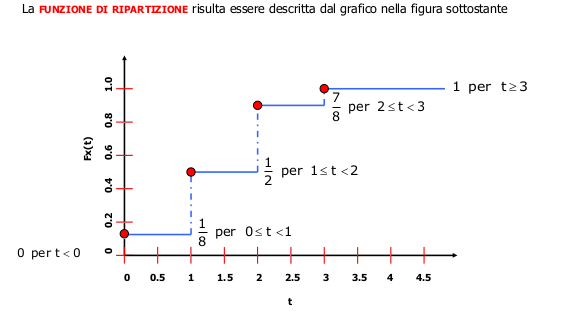
\includegraphics[scale=0.8]{img/rip.png}
\end{center}
Avendo definito la funzione di ripartizione, adesso tutte le questioni riguardanti la variabile casuale $X$
possono trovare una soluzione attraverso di essa, infatti supponiamo di calcolare $P(\{a < X \leq b\})$
con l'evento ${X \leq b}$ esprimibile come l'unione dei due eventi indipendenti ${X \leq a}$ e ${a < X \leq b}$ da cui si ricava,
usando il terzo assioma della probabilità la seguente formula:
\[ \begin{split}
        P(\{X \leq b\}) & = P(\{X \leq a\}) + P(\{a < X \leq b\}) \ \text{da cui si ricava} \\
        P(\{a < X \leq b\}) & = F(b) - F(a) \\
    \end{split} \]
Questa formula ci permette di determinare la probabilità che una variabile casuale possa assumere valori in intervalli reali
e ciò ha un notevole utilizzo in statistica e nella probabilità.

In genere la funzione di ripartizione non è nota, altrimenti tutti gli eventi della nostra vita sarebbero facilmente analizzabili
senza nessuna incertezza, per cui l'obiettivo della statistica è di determinarla o determinare le grandezza ad essa associate
mentre la probabilità e le sue applicazioni assumono che sia sempre nota.
Si dimostra che sono delle funzioni di ripartizione tutte e sole le funzioni del tipo:
\[F:\mathbb{R}\to[0,1]\]
\newpage
che godono simultaneamente delle seguenti proprietà:
\begin{itemize}
\item $F$ è monotona crescente
\item \[\lim_{t\to+\infty} F(t)=1\]
\item \[\lim_{t\to-\infty} F(t)=0\]
\item \[\lim_{t\to t_0^+} F(t)=F(t_0),\,\,\forall t_0\in\mathbb{R}\]
     fnsfgsgsjgjfskshfkj   
\end{itemize}
Le variabili aleatorie si distinguono in due categorie in base alla proprietà di continuità delle corrispondenti funzioni di ripartizione
\subsubsection{Variabile Aleatoria Discreta}
Una variabile aleatoria è detta \textbf{variabile aleatoria discreta} nel caso in cui
l'insieme dei valori $S$ che essa può assumere (supporto) è finito (ovvero costituito
da un numero finito di elementi) o costituito da una infinità di valori discreti. Ad ogni variabile aleatoria discreta si associa, oltre alla funzione di ripartizione, una funzione che fornisce delle valutazioni sulla probabilità che essa assuma specifici valori.\\
Sia $S$ il supporto della variabile aleatoria $X$. Si dice \textbf{distribuzione discreta di probabilità} la funzione:
\[p_X:\mathbb{R}\to[0,1]\]
coì definita:
\[
\begin{cases}
p(X=t)\,\,\,\,  \forall t\in S\\
0\,\,\,\,  altrimenti
\end{cases}
\]
Una funzione $p_X$ definita su un insieme finito $S$ è una distribuzione di probabilità se e solo se sono soddisfatte simultaneamente le seguenti proprietà:
\begin{itemize}
\item \[p_X(t)\geq 0\,\,\,\, t\in \mathbb{R}\]
\item \[\sum_{s\in S} p_X(s)=1\]

\newpage
questa proprietà deriva dalle due precedentemente introdotte:
\begin{itemize}
\item $P(\Omega)=1$
\item data la famiglia $\{A_i,i\in I\subseteq N\}$ 
di eventi incompatibili vale:
\[P(\bigcup_{i\in I} A_i)=\sum_{i\in I} P(A_i)\]
\end{itemize}
\end{itemize}
Tra le funzioni di ripartizione delle variabili discrete e le distribuzioni discrete di
probabilità esiste una corrispondenza biunivoca, nel senso che le une identificano
univocamente le altre. Si ha infatti che:
\begin{itemize}
\item \[F_X(t)=\sum_{s\in S:s\subseteq t} p_X(s)\,\,\, \forall t\in \mathbb{R}\]
\item \[p_X(s)=F_X(s)-\lim_{t\to s^{-}} F_X(t)\,\,\, \forall s\in S\]
\end{itemize}
Dalla prima di tali relazioni se ne deduce che le funzioni di ripartizione delle variabili
aleatorie discrete presentano dei \textit{salti} in corrispondenza dei valori \textit{s} mentre
sono costanti per gli altri valori: per tale ragione vengono dette \textit{funzioni a gradino}.
\subsubsection{Variabile Aleatoria Continua}
Una variabile aleatoria è detta continua nel caso in cui la corrispondente funzione di ripartizione $F_X$ sia continua. In particolare è detta \textbf{assolutamente continua} se esiste una funzione:
\[f_X:\mathbb{R}\to R_+\]
tale che:
\[F_X(t)=\int_{-\infty}^t f_X(u)du\,\,\,\forall t\in \mathbb{R}\]
Una tale funzione quando esista viene detta \textbf{densità di probabilità }di $X$.\\
È detto poi \textbf{supporto} della variabile $X$ l'insieme:
\[S=\{t\in\mathbb{R}:f_X(t)\neq 0\}\]
Si osservi che se la densità di probabilità di una variabile casuale esiste allora la
funzione di ripartizione è una sua primitiva.
Per semplicità supporremo nel seguito che le variabili aleatorie assolutamente
continue abbiano funzione di ripartizione derivabile e che la funzione di densità di
probabilità sia la derivata della funzione di ripartizione.\\
Come per le distribuzioni discrete di probabilità anche le funzioni di densità di
probabilità per essere tali devono soddisfare le seguenti due proprietà:
\begin{enumerate}
\item \[f_X(t)\geq 0\,\,\, \forall t\in \mathbb{R}\]
\item \[\int_{-\infty}^{+\infty}f_X(t)dt=1\]
\end{enumerate}
La probabilità che una variabile aleatoria continua (o
assolutamente continua) assuma un ben determinato valore è sempre nulla. Infatti, se $X$ è una variabile aleatoria continua allora $\forall t_0\in \mathbb{R}$ vale:
\[P(X=t_0)=P(X\leq t_0)-\lim_{t\to t_0^-}P(X\leq t)=F_X(t_0)-\lim_{t\to t_0^-} F_X(t)=F_X(t_0)-F_X(t_0)=0\]
\begin{center}
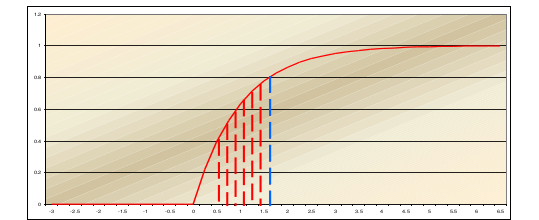
\includegraphics[scale=0.6]{img/con.png}
\end{center}
Pertanto quando si pensa a variabili aleatorie continue, non ha mai senso domandarsi, quale sia la probabilità che esse assumano valori esatti. Al contrario ha senso domandarsi quale sia la probabilità che tali variabili assumano
valori in specifici intervalli dell'asse reale.\\
Per calcolare la probabilità che una variabile casuale continua $X$ assuma un valore in un intervallo $(a,b]\subseteq \mathbb{R}$ è possibile far ricorso alla seguente formula:
\[P(X\in(a,b])=\int_a^b f_X(u)du\,\,\, \forall t\in\mathbb{R}\]
quindi:
\[P(X\in(a,b])=F_X(b)-F_X(a)=\int_{-\infty}^b f_X(u)du-\int_{-\infty}^a f_X(u)du\]
valutiamo in $b$:
\[F_X(b)=\int_{-\infty}^b f_X(u)du=P(X\leq b)\]
che è quindi l'area sottesa alla curva della funzione fino al punto $b$ sull'asse delle $x$.\\
Valutiamo anche in $a$:
\[F_X(a)=\int_{-\infty}^a f_X(u)du=P(X\leq a)\]
che è quindi l'area sottesa alla curva della funzione fino al punto $a$ sull'asse delle $x$.\\
quindi:
\[P(X\in(a,b])=F_X(b)-F_X(a)\]
è l'area sottesa alla curva della funzione fino dal punto $a$ al punto $b$ sull'asse delle $x$.\\
In pratica la probabilità che sia soddisfatto l'evento $X\in(a,b]$ corrisponde all'area sottesa dalla densità $f_X$ nell'intervallo $(a,b]$:
\begin{center}

\psscalebox{1.0 1.0} % Change this value to rescale the drawing.
{
\begin{pspicture}(0,-2.375)(8.38,2.375)
\psbezier[linecolor=black, linewidth=0.04](5.9990716,0.4275487)(5.9981446,1.2275481)(1.6000015,-0.37754923)(1.6009284,-1.1775487080233007)
\psline[linecolor=black, linewidth=0.04, arrowsize=0.05291667cm 2.0,arrowlength=1.4,arrowinset=0.0]{->}(0.8,-2.375)(0.8,2.425)
\psline[linecolor=black, linewidth=0.04, arrowsize=0.05291667cm 2.0,arrowlength=1.4,arrowinset=0.0]{->}(0.4,-1.975)(7.2,-1.975)
\psline[linecolor=black, linewidth=0.04, linestyle=dashed, dash=0.17638889cm 0.10583334cm](1.6,-1.175)(1.6,-1.975)
\psline[linecolor=black, linewidth=0.04, linestyle=dashed, dash=0.17638889cm 0.10583334cm](6.0,0.425)(6.0,-1.975)
\rput[bl](1.6,-2.375){$a$}
\rput[bl](5.6,-2.375){$b$}
\rput[bl](7.2,-2.375){$X$}
\rput[bl](-0.1,2.025){$f_X()$}
\rput[bl](6.4,-0.775){$P(X\in(a,b])$}
\psline[linecolor=black, linewidth=0.04, linestyle=dotted, dotsep=0.10583334cm](5.6,0.425)(2.0,-1.175)
\psline[linecolor=black, linewidth=0.04, linestyle=dotted, dotsep=0.10583334cm](5.6,0.025)(2.0,-1.575)
\psline[linecolor=black, linewidth=0.04, linestyle=dotted, dotsep=0.10583334cm](5.6,-0.375)(2.0,-1.975)
\psline[linecolor=black, linewidth=0.04, linestyle=dotted, dotsep=0.10583334cm](5.6,-0.775)(2.8,-1.975)
\psline[linecolor=black, linewidth=0.04, linestyle=dotted, dotsep=0.10583334cm](5.6,-1.175)(3.6,-1.975)
\psline[linecolor=black, linewidth=0.04, linestyle=dotted, dotsep=0.10583334cm](5.6,-1.575)(4.8,-1.975)
\end{pspicture}
}

\end{center}
quindi:
\[[P(X\in(a,b])=\int_a^bf_X(u)du\,\,\,\forall a,b\in\mathbb{R},\,\,\,a<b\]
inoltre essendo $P(X=a)=0$ si ha:
\[[P(X\in(a,b])=p(X\in[a,b])\,\,\,\forall a,b\in\mathbb{R},\,\,\,a<b\]

Si è visto che per definizione:
\[F_X(t)=\int_{-\infty}^tf_X(u)du\,\,\,\forall t\in\mathbb{R}\]
Ovvero che la funzione di ripartizione è la funzione integrale della funzione di densità di probabilità. Quindi, data la funzione di ripartizione, si ottiene la funzione di densità di probabilità tramite derivazione:
\[\frac{d}{dt}F_X(t)=f_X(t)\]
\end{document}
